% Chapter Template

\chapter{Enhanced Models} % Main chapter title

\label{Chapter:Ordinal_Regression} % Change X to a consecutive number; for referencing this chapter elsewhere, use \ref{ChapterX}

In this chapter we present a part of the work published in \citep{de2017deep}. Concretely, the optimized classification model for DR disease grading. The model presented here has a statistically proven ophthalmologist level performance, reaching a inter-rating agreement in never-seen-before Messidor dataset of $QWK = 0.83$, with a unique evaluation and no ensembling. 

%----------------------------------------------------------------------------------------
%	SECTION 1
%----------------------------------------------------------------------------------------

\section{Introduction}

Deep Learning (DL) methods \citep{nature-deep-learning}, \citep{888} have been extensively used in the last years for many automatic classification tasks. For the case of image classification, the usual procedure consists on extracting the important features using a set of convolutional layers and, after that, make a final classification with these features using a set of fully connected layers. At the end, a soft-max output layer gives the predicted output probabilities of belonging to the classes predefined in the model. During training, model parameters are changed using a gradient-based optimization algorithm, which minimizes a predefined loss function.\citep{Goodfellow-et-al-2016} 

Once the classifier has been trained (i.e. model layer parameters have been fixed), the quality of the classification output is compared against the correct "true" values stored on a labeled dataset. This data is considered as the gold standard, ideally coming from the consensus of the knowledge of a committee of human experts.

This mapping allows the classification of multi-dimensional objects into a small number of categories. The model is composed by many neurons that are organized in layers and blocks of layers, piled together in a hierarchical way. Every neuron receives the input from a predefined set of neurons. In addition, every connection has a parameter that corresponds to the weight of the relation. 

The function of every neuron is to make a transformation of the received inputs into a calculated output value. For each incoming connection, a weight is multiplied by the input value and the aggregation over all inputs is fed to an activation function that calculates the neuron output. Parameters are usually optimized using a stochastic gradient descent algorithm that minimizes a predefined loss function. Network parameters are updated after back-propagating the loss function gradients through the network. These hierarchical models are able to learn multiple levels of representation that correspond to different levels of abstraction, which enables the representation of complex concepts in a compressed way \citep{Bengio:2013:RLR:2498740.2498889}, \citep{bengio-2009}.

The first successful convolutional neural network (CNN) published \citep{LeCun:98} was designed for hand-written digit recognition. This early CNN implementation used a combination of convolution, pooling and non-linearity that has been the key feature of DL until now. It used convolutions for extracting spatial features, sub-sampling for reducing maps size, a non-linearity in the form of tanh or sigmoids, and a fully connected multi-layer neural network as final classifier.  Network parameters were all learned using an end-to-end optimization algorithm using stochastic gradient descent. One of the first successful implementations using GPUs was published in \citep{ciresan80deep} where they successfully trained a neural network with 9 layers, also for handwritten digit recognition. The DL breakthrough took place with the publication of \citep{NIPS2012_4824} where, for the first time, a CNN won the Imagenet\citep{imagenet_cvpr09} classification competition by a large margin. The network, named AlexNet, introduced a set of innovative techniques like data augmentation, the use of rectified linear units (ReLUs) as non-linearities, the use of dropout for avoiding overfitting, overlapping max-pooling avoiding the averaging effects of avg-pooling and the use of GPUs for speeding up the training time. This paper proved experimentally that CNNs were able to solve complex tasks. From the publication of this paper many improvements where published, like \citep{sermanet2014overfeat} with the introduction of Overfeat, a network derivation of AlexNet where they proposed learning bounding boxes, which later gave rise to many other papers on the same topic. In \citep{vggnet}, VGG networks where presented. It was the first time that small 3x3 convolution filters where used and combined as a sequence of convolutions. The previous big filters of 9x9 and 11x11 present in AlexNet started to become smaller. The great advantage of VGG network was the insight of stacking 3x3 convolutions as a substitution of large filters. These ideas were used in the design of posterior networks like ResNet and Inception. GoogleNet\citep{googlenet} and Inception \citep{szegedy2016rethinking} were the first attempts to reduce the size of big networks. DL was becoming very useful for categorization of images and video frames, but its main concern was its low efficiency in size and computation. Inception module used a parallel calculation of 1x1, 3x3 and 5x5 convolutions significantly reducing the number of operations required by networks like AlexNet and VGG. Bottleneck layers (1x1 convolutions) where used before the calculation of bigger size convolutions for reducing the number of input filters, reducing in this way the computational costs without losing generality. So, 1x1 convolutions have been proven to achieve state-of-the-art results in Imagenet classification tasks. The reason of this success is that input features are correlated, being removed by combining them appropriately with the 1x1 convolutions. Then, after convolution with a smaller number of features, they can be expanded again into a meaningful combination for the next layer. Another revolution came with the introduction of residual networks in \citep{he2016deep}. These networks used a combination of 3x3 convolutional layers with a by-pass of the input every two layers that was summed up to the output. The introduction of such bypass improved the gradient propagation through the network allowing the use of deeper networks and improving the classification capabilities. In \citep{szegedy2017inception}, a modified version of Inception networks called InceptionResNet was published to introduce this idea to such networks. Residual blocks allowed the reduction of training time, not improving significantly the classification performance. 
%\vspace{1cm} % just to get a page break. Remove if not required

DL models have been also successfully applied  in many medical classification tasks. In \citep{esteva2017dermatologist} a DL classifier was designed achieving dermatologist-level accuracy for skin cancer detection. In \citep{wentao2018deeplung} a 3D CNN for automated pulmonary nodule detection and classification was built. In \citep{wang2018classification} a CNN Alzheimer's disease classifier with high performance was also described. In \citep{doi:10.1001/jama.2016.17216} the authors presented a DR classifier with better performance than human experts in the detection of the most severe cases of the disease.

\section{Related work}\label{class2:sec:related}

Many deep learning classifiers for DR have been published in the last years. In \citep{delatorre2017} a DL classifier was published for the prediction of the different disease grades. This model was trained using the public available EyePACS dataset. The training set had 35,126 images and the test set 53,576. The quadratic weighted kappa (QWK) evaluation metric \citep{cohen1968weighted} was close to the reported by human experts in the test set using a unique DL model without ensembling. 

In \citep{doi:10.1001/jama.2016.17216} a binary DL classifier was published for the detection of the most severe cases of DR (grouping classes 0 and 1 of DR on one side, and classes 2, 3 and 4 on another). This model was trained using an extended version of the EyePACS dataset mentioned before with a total of 128,175 images and improving the proper tagging of the images using a set of 3 to 7 experts chosen from a panel of 54 US expert ophthalmologists. This model surpassed the human expert capabilities, reaching approximately a performance of 97\% in sensitivity and 93.5\% in specificity in test sets of about 10,000 images. The strength of this model was its ability to predict the more severe cases with a sensitivity and specificity greater than human experts. The drawback, as many DL based models, is its lack of interpretability. The model acts like a \emph{intuition machine} with a highly statistical confidence but lacking an interpretation of the rationale behind the decisions, making difficult to the experts to have clues to improve the diagnostics.

\section{Classification model for DR} \label{class2:sec:class}

\subsection{Data}
\label{class2:sec:data}

We use the EyePACS dataset presented in chapter \ref{Chapter:Background}. The dataset is split into two disjoint sets containing eye images of different patients, one for training and the other for testing.

The training set contains a total of $75,650$ images; $55,796$ of class 0, $5,259$ of class 1, $11,192$ of class 2, $1,805$ of class 3 and $1,598$ of class 4. The validation set used for hyper-parameter optimization has $3,000$ images; $2,150$ of class 0, $209$ of class 1, $490$ of class 2, $61$ of class 3 and $90$ of class 4. 

The test set contains a total of $10,000$ images of patients not present in training set; $7,363$ of class 0, $731$ of class 1, $1,461$ of class 2, $220$ of class 3 and $225$ of class 4. 

This dataset is not so rich and well tagged as the used in \citep{doi:10.1001/jama.2016.17216} but allows to train models near human expertise that are useful to show the purposes of our work, which is not only a good performance of the classification results but mainly to provide tools for interpretability of the final classification of each patient.

\subsection{Construction of the classifier}

The model calculates the probability $P(\mathcal{C} | \mathcal{I})$, being $\mathcal{C}$ one of the possible output classes and $\mathcal{I}$ the retina image. Using as a last layer a $SoftMax$ function over the values after the last linear combination of features. This probability is calculated as $P(\mathcal{C} | \mathcal{I}) = \frac{\me^{S_{i}}}{\sum_{j=1}^{C} \me^{S_{j}}}$. Let us call $S_{C}$ the score of class $C$, being $S_C$ the final value of each output neuron before applying the $Softmax$. $Softmax$ function is required for calculating the probability of every class, but in case of being interested only on $argmax(Softmax)$, we do not need evaluate $Softmax$ because $argmax(S_i) = argmax(Softmax(S_i))$. Thus, we skip $Softmax$ from the interpretation analysis.

\subsubsection{Design guidelines for DR classification} \label{class_guidelines}

Up to now, the design of deep neural network models is mainly driven  by experience. Nowadays it is still more an art than a science and lacks a systematic way for designing the best architecture for solving a problem. In previous works (see \citep{jdelatorre2016} and \citep{delatorre2017}), we have tested different kinds of architectures for DR classification. Using the previous experience in such works we report here a set of guidelines that have been used to build the proposed classification model for DR. These design principles for DR classification can be summarized into: use an optimal image resolution, use all the image information available, use a fully CNN, use small convolutions, adapt the combination of convolution sizes and number of layers to have a final RF as similar as possible to the image size, use ReLU as activation function, use batch normalization in every layer, use QWK as a loss function, use a efficient number of features and use a linear classifier as the last layer.

\paragraph{Use an optimal image resolution} On the one hand, image input size has a great importance in the classification results. For this problem, other papers like \citep{jdelatorre2016} have shown that better results can be achieved with retina diameters of 512 pixels than with 384, 256 or 128 pixels. Some tests done using densities larger than 512 pixel/diameter seem to not improve significantly the classification rates. On the other hand, the hardware of calculation devices fix a limitation on the available resources. Input image size has a great impact on the memory and calculation time required for the training and test of the deep neural network models. For this present work, we tested models of 128, 256, 384, 512, 640, 724, 768 and 892 pixels of retina diameter. With this dataset, diameters greater than 640 does not seem to report better results. The optimal size is a retina diameter equal to 640 pixels. This is the one used for the results shown in this chapter.

\paragraph{Use all the available image information} In previous studies published in \citep{jdelatorre2016}, due to hardware limitations, the classification models were designed using limited input information, using only part of the available input, requiring ensembling solutions to combine the results from evaluating different parts of the same retina. A 512x512 input image model was used with a random selection of a rotated square (diagonal equal to the retina diameter). In this way only a 64\% of the retina information available was used in the classification prediction. On test time, five rotated versions of the input where averaged in order to get a better evaluation result. In this chapter, we use a network that receives all the input information available not requiring ensembling on test time. Only background located further from the diameter is removed.

\paragraph{Use a fully convolutional neural network} CNNs are computationally more efficient than fully connected ones. CNNs are ideal for exploiting the typical high local pixel correlations present in images.

\paragraph{Use small size convolutions} Spatial convolutions are very expensive in memory and time requirements, growing both quadratically with kernel size. Papers \citep{vggnet}, \citep{he2016deep},  \citep{szegedy2016rethinking} proved experimentally that stacking small convolution layers and increasing depth is possible to obtain better results than using convolutions of bigger size with less depth. In \citep{eldan2016power} and \citep{cohen2016expressive} theoretical studies proved also that model expressiveness grows exponentially with depth. In our chapter, we follow a similar approach to the one used in \citep{vggnet} using exclusively 3x3 convolutions in every feature layer. Even convolution sizes are discarded due to its asymmetry when used with zero padding.

\begin{figure}[ht!]
	\centering
	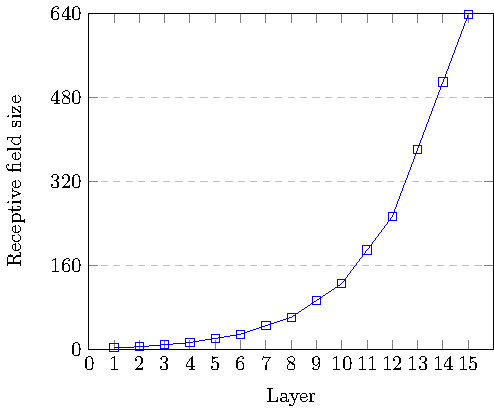
\includegraphics[width=0.50\textwidth]{Figures/chapter_classification/figures/receptive_field_640.pdf}
	\caption{Model RF growth}
	\label{class2:fig:rf_graph}
\end{figure}

\paragraph{Adapt convolution sizes and number of layers to get a RF as similar as possible to the image size} One important aspect of CNNs is the RF size. RF defines the theoretical space covered by a convolution in the input-space. The ideal case is having a RF in the last layer equal to the image size, because in such a way we are sure that all the information available is used. RFs greater than image size are inefficient, for this reason sometimes can be necessary to slightly modify the convolution sizes of some layer to get the desired one. Figure \ref{class2:fig:rf_graph} shows the RF growth of our model.

\paragraph{Use rectified linear unit (ReLU) as activation function} ReLU is a computationally efficient activation function that is very suitable to be used with very deep CNNs\citep{Dahl2013}. We have tested other activation functions such as LeakyReLU, ELU and SeLU reporting similar and even worse results, introducing complexity to the model without adding any significant advantage to the final result.

\paragraph{Use batch normalization in every layer} Batch normalization \citep{batch-norm} stabilize the training and accelerates convergence. In this application there is a great difference between using batch normalization or not. To the point that not using it makes very difficult or even impossible the training.

\paragraph{Use QWK as a loss function} For multi-class classification the standardized loss function to use is the logarithmic loss \citep{Goodfellow-et-al-2016}. In \citep{delatorre2017} it is shown that for ordinal regression problems, where not only a multi-class classification is taking place but also it is possible to establish a sorting of the classes based on some hidden underlying causes, QWK-loss can also be used with better results. The properties of this function as a loss function have been widely studied in \citep{delatorre2017}. The difference in performance of the final results is very high. Optimizing directly QWK allows achieving better classification results.

\paragraph{Use a linear classifier as a last layer} For simplicity and interpretability, we expect the model to disentangle completely the features required for the classification. Final classification is required to be done using a linear combination of last layer features.

\begin{figure}[ht!]
	\centering
	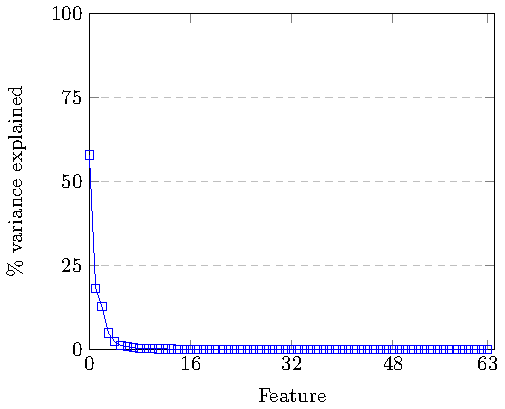
\includegraphics[width=0.50\textwidth]{Figures/chapter_classification/figures/PCA_feature_space.pdf}
	\caption{Feature space cummulative PCA variance of training set}
	\label{class2:fig:pca_graph}
\end{figure}

\paragraph{Use a efficient number of features} With infinitely number of resources we can use a big network. In our project we have limited device resources. In addition, we would like to be able to implement the result in devices with low resources too. Having this in mind, we tested networks of different sizes. In order to check the redundancy of information, we made a principal component analysis (PCA) in the feature space of the last layer, arriving to the conclusion that about 32 of the features explain 98.3 \% and 48 features, 99.997\% of the total variance. We studied different configurations using different number of features from 512 to 32. Values of 32 showed a reduction in performance that increased when using 64 features. Higher number of features did not improve the results. In figure \ref{class2:fig:pca_graph} we show the variance explained by the 64 feature vector space.

\subsubsection{Classification model description}

Following the given guidelines, our model uses a 3x640x640 input image obtained from a minimal preprocessing step, where only the external background borders are trimmed and later resized to the required input size. Figure \ref{class2:fig:drmodel} shows a block diagram of the model. It is a CNN with 391,325 parameters, divided in 17 layers. Layers are divided into two groups: the feature extractor and the classifier. The feature extraction has 7 blocks of 2 layers. Every layer is a stack of a 3x3 convolution with stride 1x1 and padding 1x1 followed by a batch normalization and a ReLU activation function. Between every block a 2x2 max-pooling operation of stride 2x2 is applied. After the 7 blocks of feature extraction, the RF of the network has grown till reaching 637x637, that is approximately equal to the input size 640x640 (see fig \ref{class2:fig:rf_graph} to see the RF of every layer). Afterwards, the classification phase takes place using a 2x2 convolution. A 4x4 average-pooling reduces the dimensionality to get a final 64 feature vector that are linearly combined to obtain the output scores of every class. A soft-max function allows the conversion of scores to probabilities to feed the values to the proper cost function during the optimization process. The feature extractor has 16 filters in the first block, 32 in the second and 64 in all the other.

\subsection{Training procedure}

As presented in section \ref{class2:sec:data}, the training set training set has 75,650 images and the validation set used for hyper-parameter selection 3,000. Notice that the image set is highly imbalanced. In order to facilitate the learning, the training set is artificially equalized using data augmentation techniques \citep{Krizhevsky:2012} based on $0-180^{\circ}$ random rotation, X and Y mirroring and contrast\&brightness random sampling.

A random initialization based in the Kaiming\&He approach \citep{kaiming} is used. All models are optimized using a batch based first order optimization algorithm called Adam \citep{DBLP:journals/corr/KingmaB14}. The loss function used for optimizing the model is the QWK-loss function, with a batch size of $15$ and a learning rate of $3x10^{-4}$ \citep{delatorre2017}. For every batch, the images are chosen randomly from the training set, with repetition. 

After network training, a linear classifier formed by the combination of the 128 features of the two eyes of the patient is trained. In this way is possible to increase further the prediction performance of the model using all the information available of the patient.

\begin{figure}[ht!]
	\centering
	\scalebox{0.9}{
		\begin{subfigure}[b]{.31\textwidth}
			\centering
			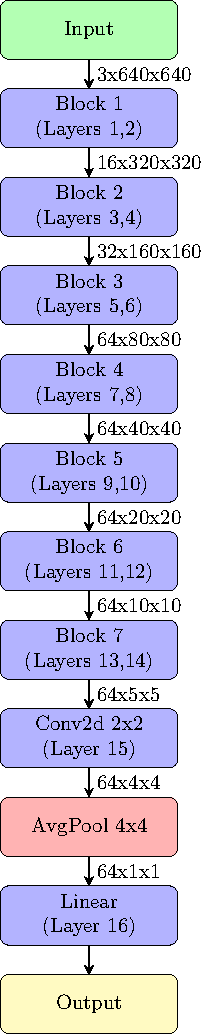
\includegraphics[width=\textwidth]{Figures/chapter_classification/figures/model640.pdf}
			%\caption{Full classification stack}	
		\end{subfigure}
		\hfill    
		\begin{subfigure}[b]{.30\textwidth}
			\centering
			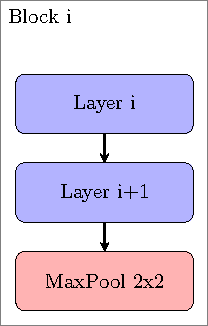
\includegraphics[width=\textwidth]{Figures/chapter_classification/figures/modelblock.pdf}\\
			\vspace{2cm}
			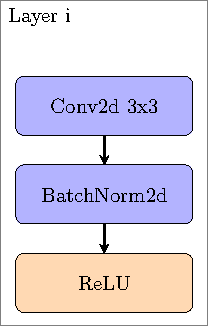
\includegraphics[width=\textwidth]{Figures/chapter_classification/figures/modellayer.pdf}\\
			\vspace{2cm}
			%\caption{Block and layer constituents}
		\end{subfigure}
	}
	\hfill 
	\caption[Prediction model]{Prediction model of 391,325 trainable parameters (located in blue blocks).}  
	\label{class2:fig:drmodel} 
\end{figure}

\section{Results}\label{class2:sec:results}

The model is trained for 300 epochs, reaching a QWK value of $0.814$ on the validation set. The value achieved in the testing set (with images not used in the training) of 10,000 images is of $0.801$. Using a linear classifier for combining the features of both eyes $QWK_{test}$, we can reach a QWK value of $0.844$. Expert ophthalmologist report QWK inter-rating agreement values close to $0.80$. 

If we consider a binary classification with two categories, one for severe cases of DR (grouping classes 2, 3 and 4) and another for non-sever cases (classes 0 and 1), we can calculate the usual classification evaluation metrics. Over EyePACS test set we obtain the following values for different measures\footnote{\label{class2:footn:notation} Notation: N: sample size, TP: true positives, TN: true negatives, FP: false positives, FN: false negatives, CI: confidence interval, PPV: positive predictive value, NPV: negative predictive value, $F_1$: F1 score and MCC: Matthews correlation coefficient}: N=10,000, TP=1,727, TN=6,859, FP=1,235, FN=179, Sensitivity=0.906 (95\% CI: 0.893 to 0.919), Specificity=0.847 (95\% CI: 0.840-0.855), PPV=0.583, NPV=0.975, Accuracy=0.857, $F_1$=0.710 and MCC=0.648.

For comparison purposes with other works, we tested also our model against the standardised Messidor-2 dataset \citep{decenciere_feedback_2014}. We achieve a $QWK$ of $0.832$ for this dataset. Binary classification statistics for prediction of the most severe cases of DR (grouping classes 2, 3 and macular edema) are: N=1200, TP=465, TN=627, FP=61, FN=47, Sensitivity=0.908 (95\% CI: 0.883 to 0.933), Specificity=0.911 (95\% CI: 0.890-0.933), PPV=0.884, NPV=0.930, Accuracy=0.910, $F_1$=0.896 and MCC=0.817. 

We can see that the results obtained with the Messidor-2 dataset are better because of the improved quality of images in the dataset and a also a better labelling of the examples.


In order to compare our model with  state-of-the-art \citep{doi:10.1001/jama.2016.17216}, table \ref{class2:tab:bench} show statistics for prediction of the most severe cases of DR (classes 2, 3 or macular edema) for Messidor-2 Dataset. We see that with a two orders of magnitude smaller model, it is possible to obtain good enough values of sensitivity and specificity. Our model is designed to be simple enough to be run is low resources devices, like mobile phones, with good performance. Furthermore, model simplicity eases the score calculations required for generating explanations.

\begin{table}[ht]
	\centering
	\scalebox{1.0}{
	\begin{tabular}{crrrr}
		\hline
		Reference & Parameters & Depth & Sensitivity & Specificity\\ \hline
		(Gulshan et al., 2016) & $23,851,784$ & 159 & 96.1 \% & 93.9 \% \\ 
		Our work & $391,325$ & 17 & 91.1 \% & 90.8 \% \\
		\hline	
	\end{tabular}
	}
	\caption{Prediction performance \& model complexity comparison of our proposal vs the state-of-the-art model (Messidor-2 data set)}
	\label{class2:tab:bench} 
\end{table}

Building a multi-class classification model needs to account for the encoding of required features for distinguishing between the different disease severity levels. This is is more difficult than a binary classifier, since it has to differentiate between more levels of DR severity. Thus, training the model for an aggregated detection (grouping the positive classes) increases the accuracy of the classifier, at the prize of missing the coding of important features that separate positive classes (1 to 4).

In our case, ophthalmologists want to distinguish all levels of severity since the treatment can be then personalized to each patient with more detail. Therefore, our goal is to make the model learn such differences in order to visualize them in the explanation model. For this reason, it is better to use all the information available about the gradation of disease (intermediate classes) in order to force the model to encode the required features that allow to separate the intermediate classes, even at the prize of reducing accuracy in the correct predictions. In this way after back-propagating the explanations, we could get the scores that the model report in the evaluation of the different classes for the same image, allowing the expert to get more knowledge about the image detection of DR signs.

\section{Conclusions}\label{class2:sec:conclusions}

We designed a model for DR classification, reaching more than 90\% of sensitivity and specificity for the detection of the more severe cases of DR, not far from the state-of-the-art solution with two orders of magnitude less parameters. The designed model is also able to differentiate between the five standardized levels of disease severity, achieving in the test set of the EyePACS dataset a quadratic weighted kappa of 0.80 with the information of one eye and of 0.844 using the information coming from both eyes. In the Messidor-2 dataset the value of QWK achieved is of 0.83 using only the information of one eye. In all cases, the achieved performance is similar or even better than the reported by experts ophthalmologists, that is also near 0.80.

%\vspace{1cm} % just to get a page break. Remove if not required